% Main file. Compile with: latexmk -pdf main.tex   (pdfLaTeX, Overleaf-compatible; set this file as "Main document").
% Numbers in the text come from results/macros.tex and results/macros_stack.tex (generated by code/make_figures*.py).
\documentclass[11pt,a4paper]{article}
\usepackage{lmodern}
\usepackage[T1]{fontenc}
\usepackage[utf8]{inputenc}
\usepackage[margin=2.3cm]{geometry}
\usepackage{amsmath,amssymb}
\usepackage{graphicx,booktabs,tabularx,array,float,xcolor,microtype,enumitem}
\usepackage[font=small,labelfont=bf]{caption}
\usepackage{listings}
\usepackage{tikz}
\usetikzlibrary{arrows.meta,positioning,fit,calc}
\usepackage[colorlinks=true,linkcolor=blue!50!black,citecolor=blue!50!black,urlcolor=blue!50!black]{hyperref}
\graphicspath{{figures/}}
\newcommand{\collAnormal}{4.0 \pm 0.4}
\newcommand{\collAhazard}{19.7 \pm 1.6}
\newcommand{\collAhard}{18.9 \pm 1.7}
\newcommand{\gapAhazard}{1.26 \pm 0.04}
\newcommand{\passAnormal}{96.0 \pm 0.4}
\newcommand{\collBnormal}{4.2 \pm 1.2}
\newcommand{\collBhazard}{8.2 \pm 0.6}
\newcommand{\collBhard}{8.9 \pm 0.7}
\newcommand{\gapBhazard}{1.68 \pm 0.07}
\newcommand{\passBnormal}{95.8 \pm 1.2}
\newcommand{\collCnormal}{4.0 \pm 0.7}
\newcommand{\collChazard}{20.2 \pm 1.4}
\newcommand{\collChard}{19.2 \pm 1.0}
\newcommand{\gapChazard}{1.23 \pm 0.05}
\newcommand{\passCnormal}{96.0 \pm 0.7}
\newcommand{\collDnormal}{4.3 \pm 0.5}
\newcommand{\collDhazard}{21.3 \pm 1.8}
\newcommand{\collDhard}{20.3 \pm 1.7}
\newcommand{\gapDhazard}{1.14 \pm 0.03}
\newcommand{\passDnormal}{95.7 \pm 0.5}
\newcommand{\expertnormal}{0.0}
\newcommand{\experthazard}{0.4}
\newcommand{\experthard}{0.5}
\newcommand{\expertgap}{1.57}
\newcommand{\diagnormalAcoll}{3.9}
\newcommand{\diagnormalExcoll}{0.0}
\newcommand{\diagnormalOL}{7.4}
\newcommand{\diagunguidedAcoll}{4.0}
\newcommand{\diagunguidedExcoll}{0.0}
\newcommand{\diagunguidedOL}{6.3}
\newcommand{\diagguidedAcoll}{38.0}
\newcommand{\diagguidedExcoll}{0.1}
\newcommand{\diagguidedOL}{48.3}
\newcommand{\diaguniformAcoll}{9.2}
\newcommand{\diaguniformExcoll}{0.4}
\newcommand{\diaguniformOL}{21.4}
\newcommand{\nvMAE}{0.20}
\newcommand{\nvRMSE}{1.24}
\newcommand{\nvWithin}{96.7}
\newcommand{\nvMAEstatic}{0.40}
\newcommand{\nvPedRays}{142}
\newcommand{\nvAllRays}{9024}
\newcommand{\nvMAEped}{0.77}
\newcommand{\nvWithinPed}{83.8}
\newcommand{\nvMAEstaticped}{19.98}
\newcommand{\wiAgree}{96.2}
\newcommand{\wiCollReal}{19.2}
\newcommand{\wiCollTwin}{15.4}
\newcommand{\wiGapMAE}{0.10}
\newcommand{\wiGapCorr}{0.99}
\newcommand{\wiXMAE}{0.53}
\newcommand{\wiCollNoPed}{32.7}
\newcommand{\wiNcfg}{52}
\newcommand{\nerfRays}{45184}
\newcommand{\nerfIters}{5000}
\newcommand{\nerfFit}{247}
\newcommand{\nSeeds}{5}
\newcommand{\nNormal}{1500}
\newcommand{\nGen}{1200}
\newcommand{\guidanceLam}{8}
\newcommand{\nHard}{633}

\newcommand{\treeStates}{32}
\newcommand{\treeProps}{6}
\newcommand{\bmcN}{18000}
\newcommand{\bmcViol}{0}
\newcommand{\stackAColl}{23.0}
\newcommand{\stackAPass}{77.0}
\newcommand{\stackBTColl}{2.0}
\newcommand{\stackBTPass}{98.0}
\newcommand{\stackBTGap}{1.88}
\newcommand{\stackBToColl}{0.0}
\newcommand{\stackBToPass}{100.0}
\newcommand{\stackBToGap}{1.80}
\newcommand{\stackPlColl}{10.0}
\newcommand{\stackPlPass}{90.0}
\newcommand{\stackPlGap}{1.92}
\newcommand{\stackPsColl}{2.0}
\newcommand{\stackPsPass}{98.0}
\newcommand{\stackPsGap}{2.46}
\newcommand{\plrmstrack}{0.07}
\newcommand{\plrmsacc}{2.40}
\newcommand{\pljerkNF}{14.22}
\newcommand{\pljerklat}{19.15}
\newcommand{\pljerksm}{5.75}
\newcommand{\pltpass}{9.56}
\newcommand{\btFullHz}{3.2}
\newcommand{\btFullNorm}{2.4}
\newcommand{\trFFRms}{0.068}
\newcommand{\trFFColl}{21.7}
\newcommand{\trFFJerk}{13.6}
\newcommand{\trFFmRms}{0.073}
\newcommand{\trFFmColl}{20.0}
\newcommand{\trFFmJerk}{12.1}
\newcommand{\trPDRms}{0.064}
\newcommand{\trPDColl}{23.3}
\newcommand{\trPDJerk}{19.0}
\newcommand{\trPDmRms}{0.068}
\newcommand{\trPDmColl}{21.7}
\newcommand{\trPDmJerk}{16.4}
\newcommand{\nsJerk}{19.2}
\newcommand{\nsColl}{21.7}
\newcommand{\fNoneplain}{3.0}
\newcommand{\fNonemonitor}{3.0}
\newcommand{\fdropoutplain}{8.0}
\newcommand{\fdropoutmonitor}{4.2}
\newcommand{\fstuckplain}{4.5}
\newcommand{\fstuckmonitor}{2.0}
\newcommand{\fbiasplain}{1.8}
\newcommand{\fbiasmonitor}{1.8}
\newcommand{\flatencyplain}{2.0}
\newcommand{\flatencymonitor}{1.5}
\newcommand{\fbrakeplain}{8.5}
\newcommand{\fbrakemonitor}{8.2}
\newcommand{\embFlns}{9.0}
\newcommand{\embFlflash}{33.5}
\newcommand{\embFlerr}{2.9e-06}
\newcommand{\embFln}{4.1}
\newcommand{\embFlh}{20.5}
\newcommand{\embIqns}{9.3}
\newcommand{\embIqflash}{9.2}
\newcommand{\embIqerr}{5.7e-06}
\newcommand{\embIqn}{4.5}
\newcommand{\embIqh}{22.1}
\newcommand{\embParams}{8449}
\newcommand{\embMacs}{8320}


\setlength{\parskip}{3pt}
\renewcommand{\arraystretch}{1.12}
\newcolumntype{Y}{>{\raggedright\arraybackslash}X}
\lstdefinestyle{py}{language=Python,basicstyle=\ttfamily\scriptsize,numbers=left,numberstyle=\tiny\color{gray},
  breaklines=true,frame=single,rulecolor=\color{black!25},keywordstyle=\color{blue!60!black},
  commentstyle=\color{green!40!black},stringstyle=\color{orange!70!black},columns=fullflexible,
  showstringspaces=false,tabsize=4,xleftmargin=1.5em,aboveskip=6pt,belowskip=6pt}
\lstdefinestyle{plain}{basicstyle=\ttfamily\footnotesize,frame=single,rulecolor=\color{black!25},columns=fullflexible,breaklines=true}
\newcommand{\done}{\textbf{Completed}}
\newcommand{\planned}{\textbf{Planned}}
\newcommand{\unrun}{\textbf{Written, not executed}}
\newcommand{\Rmax}{R_{\max}}

\title{\textbf{Simulated Self-Driving Car:\\Digital Twin, Synthetic Edge Cases and a\\Verified, Fault-Tolerant Planning Stack}}
\author{Vishwas N.\\ M.Tech, Digital Electronics and Communication, M.S.\ Ramaiah Institute of Technology (MSRIT)}
\date{\today}

\begin{document}
\maketitle
\begin{abstract}
\noindent A pedestrian-crossing world with a lidar-equipped car is used to build and test (i) a NeRF-style spacetime digital twin for ``what-if'' replay, (ii) a guided diffusion model that synthesises rare hazards, (iii) a behaviour tree with exhaustive and bounded model-checking, (iv) a space-time lattice planner with trajectory optimisation and PD tracking, (v) fault injection with a health monitor, and (vi) C export of the learned policy. Everything is pure NumPy with hand-derived gradients. Measured results: the twin agrees with the real simulator on collision outcome in $\wiAgree\%$ of \wiNcfg\ what-if cases; guided edge-case data lowers the learned policy's hazard-set collision rate from $\collAhazard\%$ to $\collBhazard\%$; the behaviour tree passes all $\treeProps$ properties in all $\treeStates$ abstract states and has $\bmcViol$ violations in $\bmcN$ bounded-model-check scenarios; with lidar perception it collides in $\btFullHz\%$ of the 800 hazard scenarios. CARLA, public datasets and on-target embedded timing are \emph{not} yet run (Section~\ref{sec:planned}).
\end{abstract}

\tableofcontents
\section{Objectives and status}
\begin{enumerate}[leftmargin=*,itemsep=1pt]
\item Replay logged drives as an editable digital twin and test ``what-if'' variants of a dangerous event.
\item Generate rare, avoidable hazards with a diffusion model and measure whether they make a learned policy safer.
\item Build a rule-based behaviour tree (BT) that is formally checked, then compare it with a learned policy and a planner.
\item Add trajectory optimisation, tracking control, fault injection and a sensor/brake health monitor.
\item Export the policy to dependency-free C and measure size, latency and int8 accuracy.
\item Document a safety argument whose claims point to measured evidence.
\end{enumerate}
\begin{table}[H]\centering\small
\begin{tabularx}{\linewidth}{lYY}\toprule
Item & Status & Evidence\\\midrule
Simulator, expert, DAgger policy & \done & Sec.~\ref{sec:e1}\\
NeRF-style twin, what-if replay & \done & Sec.~\ref{sec:e2}\\
Diffusion edge cases (\nSeeds\ seeds) & \done & Sec.~\ref{sec:e1}\\
BT verification (exhaustive + bounded) & \done & Sec.~\ref{sec:e3}\\
Lattice planner, optimisation, PD tracking & \done & Sec.~\ref{sec:e4}\\
Fault injection + monitor (5 faults) & \done & Sec.~\ref{sec:e5}\\
C export, host latency, int8 accuracy & \done\ (host CPU only) & Sec.~\ref{sec:e6}\\
KITTI-format dataset adapter & \done\ (unit test on synthetic file only) & Sec.~\ref{sec:e7}\\
Behaviour tree in CARLA & \unrun & \texttt{carla\_bt.py}; Sec.~\ref{sec:planned}\\
Real datasets (KITTI, nuScenes, Waymo) & \planned & Sec.~\ref{sec:planned}\\
On-target microcontroller timing & \planned & Sec.~\ref{sec:planned}\\\bottomrule
\end{tabularx}
\caption{Status of every item. Only ``Completed'' items have results in this report.}
\end{table}

\section{System architecture}
\begin{figure}[H]\centering
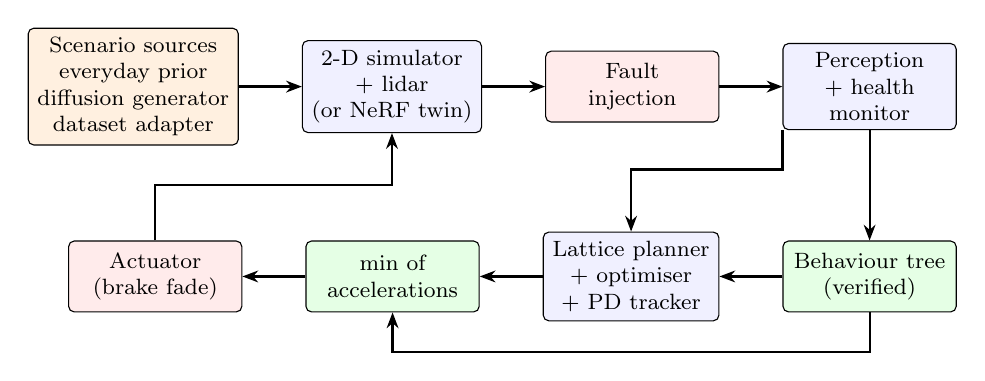
\begin{tikzpicture}[font=\footnotesize,node distance=7mm and 8mm,
  b/.style={draw,rounded corners=2pt,align=center,minimum height=9mm,minimum width=22mm,fill=blue!6},
  s/.style={b,fill=orange!12},g/.style={b,fill=green!10},r/.style={b,fill=red!8},
  a/.style={-{Stealth[length=2mm]},thick}]
\node[s](scen){Scenario sources\\everyday prior\\diffusion generator\\dataset adapter};
\node[b,right=of scen](sim){2-D simulator\\+ lidar\\(or NeRF twin)};
\node[r,right=of sim](flt){Fault\\injection};
\node[b,right=of flt](per){Perception\\+ health\\monitor};
\node[g,below=14mm of per](bt){Behaviour tree\\(verified)};
\node[b,left=of bt](pl){Lattice planner\\+ optimiser\\+ PD tracker};
\node[g,left=of pl](min){min of\\accelerations};
\node[r,left=of min](act){Actuator\\(brake fade)};
\draw[a](scen)--(sim);\draw[a](sim)--(flt);\draw[a](flt)--(per);
\draw[a](per)--(bt);\draw[a](per.south west)--++(0,-5mm)-|(pl.north);
\draw[a](bt)--(pl);\draw[a](pl)--(min);
\draw[a](bt.south)--++(0,-5mm)-|(min.south);
\draw[a](min)--(act);\draw[a](act.north)--++(0,7mm)-|(sim.south);
\end{tikzpicture}
\caption{Closed loop. The BT acts as a safety supervisor: the final command is the smaller of planner and BT accelerations.}
\end{figure}
\paragraph{Folder structure.}
\begin{lstlisting}[style=plain]
sdc_project/
  main.tex  Makefile  requirements.txt
  sections/   01_overview ... 07_appendix.tex   (one file per topic)
  code/       nn sim driving scenario_gen nerf2d stack datasets carla_bt embedded
              run_experiments run_twin run_stack make_figures make_figures_stack tests paths .py
  results/    *.json *.npz macros.tex macros_stack.tex   (generated)
  figures/    *.pdf *.png                                 (generated)
  logs/ build/                                            (generated)
\end{lstlisting}

\section{Methodology}
\subsection{World, sensor, scenarios}
The ego car (4.5\,m $\times$ 1.9\,m) drives along $+x$ with longitudinal control only ($a\in[-8,3]$\,m/s$^2$, $\Delta t=0.1$\,s, 18\,s). A pedestrian waits at $y=+5.5$\,m, possibly behind a parked car, and crosses at $x=\texttt{dist}$. A 64-ray lidar ($120^\circ$, 40\,m) adds Gaussian range noise and ray dropout. A scenario is $z=(v_0,\texttt{dist},s,\tau,o,r,p_{\rm drop},\sigma)$ with $\tau$ the pedestrian's arrival offset at the lane centre relative to the ego's constant-speed arrival ($\tau\approx0$: collision course). Collision: $\mathrm{gap}=d(\text{ego rectangle},\text{pedestrian centre})-r\le 0$. Everyday data make hazards rare (15\% of $\tau$ within $\pm3$\,s); the hazard test set keeps uniformly drawn scenarios that collide if the ego does not react.

\subsection{Learned policy (DAgger)}
MLP $65\!\to\!64\!\to\!64\!\to\!1$ on min-pooled lidar, its temporal difference and speed; trained on expert labels with DAgger (rounds with expert mixing $\beta=1,0.5,0$), MSE loss, Adam.

\subsection{NeRF-style spacetime twin}
A ray with samples $r_i$, $\delta_i=r_{i+1}-r_i$ renders the expected hit range
\begin{equation}\hat D=r_1+\sum_{i}E_i\delta_i,\quad E_i=\exp\Big(-\sum_{j\le i}\sigma_j\delta_j\Big),\qquad \frac{\partial\hat D}{\partial\sigma_k}=-\delta_k\sum_{i\ge k}E_i\delta_i .\end{equation}
Density is $\sigma(x,y,t)=\sigma_s(x,y)+\sigma_d(x,y,t)$, each $=20\,\mathrm{softplus}(\mathrm{MLP}(\text{interpolated feature grid}))$. Querying $\sigma_d$ at $t+\Delta$ shifts the pedestrian in time; the policy is then driven closed-loop on rendered lidar.

\subsection{Diffusion edge cases with guidance}
A DDPM ($T{=}200$) on normalised $z$ minimises $\|\epsilon-\epsilon_\theta(x_t,t)\|^2$. A surrogate $g_\phi(x_t,t)$ predicts the baseline policy's normalised minimum gap; sampling uses
\begin{equation}\tilde\epsilon=\epsilon_\theta+\lambda\sqrt{1-\bar\alpha_t}\,\nabla_{x_t}g_\phi(x_t,t),\qquad \lambda=\guidanceLam .\end{equation}

\subsection{Behaviour tree and verification}
Priority selector: (1) emergency brake $a=-a_b$; (2) brake to stop line $a=\min\!\big(a_{\rm cruise},-\mathrm{clip}(1.3\,a_{\rm req}+0.3,0,a_b)\big)$; (3) yield $a=\min(a_{\rm cruise},0)$; (4) cruise to 12\,m/s (8 near an occluder, 4 if the sensor is unhealthy, 6 if brakes are degraded). Here $a_{\rm req}=v^2/(2d)$, $d$ is the distance to a stop line before the pedestrian, and $a_b\in\{8,4\}$ the braking capability. A conflict is predicted from the pedestrian's entry/exit times with margins $(0.3,0.8)$\,s; a pedestrian waiting at the curb is assumed to start at 3.5\,m/s.
\emph{Verification.} (a) Exhaustive: all $\treeStates$ abstract states (hazard level $\times$ occluder $\times$ sensor flag $\times$ $a_b$), running the real action code, against $\treeProps$ properties (Table~\ref{tab:tree}). (b) Bounded model check: simulate the tree with true pedestrian state on a grid of $v_0\in\{6..14\}$, \texttt{dist}, $s\in\{0.8..3.5\}$, $\tau\in[-6,6]$ (step 0.5), occluder, $r\in\{0.25,0.6,1.0\}$: $\bmcN$ scenarios. This is a finite grid, not a proof for all continuous inputs.

\subsection{Lattice planner, optimisation, tracking}
Layered dynamic programming over $(t,s,v)$ nodes (0.5\,s layers, 6\,s horizon, $a\in\{-6,-3,-1.5,0,1,2\}$) with edges rejected if the predicted pedestrian comes within 1\,m; cost per edge $\Delta t\big[(v_d-\bar v)^2+0.15a^2\big]$. The lattice path $s^{\rm lat}$ is refined by
\begin{equation}\min_s \|s-s^{\rm lat}\|^2+\lambda_j\|\dddot s\|^2\ \ \text{s.t. } |s_k-s^{\rm lat}_k|\le0.4\,\mathrm{m},\ \lambda_j=2\!\cdot\!10^{-5},\end{equation}
solved as a linear system then clipped to the tube. Tracking: $a=a_{\rm ref}+k_p(s_{\rm ref}-s)+k_d(v_{\rm ref}-v)$ ($k_p{=}2,k_d{=}2.5$) through a first-order actuator lag (0.25\,s). Replanning at 2\,Hz.

\subsection{Fault injection and monitor}
Faults start 1\,s before the pedestrian begins to cross: \emph{dropout} (all rays lost, 2\,s), \emph{frozen frame} (2\,s), \emph{range bias} ($\times1.25$, persistent), \emph{latency} (0.3\,s, persistent), \emph{brake fade} (decel $\ge-4$\,m/s$^2$, persistent). Monitor: sensor flagged unhealthy for 2\,s if $>30\%$ of wall rays read beyond the known wall by 1.5\,m or the frame is bit-identical to the previous one; brakes flagged degraded if achieved deceleration $<70\%$ of a hard command.

\subsection{Embedded export}
Per-tensor symmetric int8 weights $q=\mathrm{round}(W/s)$, $s=\max|W|/127$, float activations; generated C has no libraries.

\section{Implementation}
All code is in \texttt{code/} (NumPy and Matplotlib only; Python 3.10+). Complete listings are in Appendix~\ref{app:code}.
\begin{table}[H]\centering\small
\begin{tabularx}{\linewidth}{lY}\toprule
File & Role\\\midrule
\texttt{nn.py} & MLP with manual back-propagation, Adam\\
\texttt{sim.py} & batched simulator, lidar, scenario samplers, open-loop hazard test\\
\texttt{driving.py} & privileged expert, DAgger, evaluation\\
\texttt{nerf2d.py} & spacetime neural field, volume rendering, twin simulator\\
\texttt{scenario\_gen.py} & DDPM over scenarios, surrogate, guidance\\
\texttt{stack.py} & behaviour tree, perception, monitor, fault injection, lattice planner, optimiser, tracker\\
\texttt{embedded.py} & C export (float32/int8), host benchmark, int8 closed loop\\
\texttt{datasets.py} & KITTI tracking labels $\to$ scenario vectors\\
\texttt{carla\_bt.py} & same BT driving a CARLA vehicle (needs CARLA server)\\
\texttt{run\_experiments.py}, \texttt{run\_twin.py}, \texttt{run\_stack.py} & experiments E1, E2, E3--E5\\
\texttt{make\_figures*.py} & figures and LaTeX number macros\\
\texttt{tests.py}, \texttt{paths.py} & smoke tests, output folders\\\bottomrule
\end{tabularx}
\caption{Code base.}
\end{table}
\paragraph{Run.}
\begin{lstlisting}[style=plain]
pip install -r requirements.txt
make test       # smoke tests
make results    # E1-E6, about 15 min on 2 CPU cores, writes results/ and logs/
make figures    # writes figures/ and results/macros*.tex
make pdf        # compiles this report (or upload the folder to Overleaf)
\end{lstlisting}
\paragraph{Design points.} Every scenario batch is vectorised, so thousands of episodes run at once; the BT is vectorised (each node returns a status array); all experiments are seeded. Perception removes the known parked car using the static map, clusters the remaining returns, and estimates pedestrian velocity by a least-squares line over the last 1\,s; with $<4$ valid samples it assumes a crossing at 1.5\,m/s (pessimistic).

\section{Completed experiments}
All numbers are produced by the code in this project (\texttt{results/*.json}); sandbox: 2 CPU cores, no GPU. Test sets are fixed and independent of every generator: 800 everyday scenarios, 800 hazard scenarios (collide if the ego does not react), and the hard-perception subset (\nHard\ scenarios with dropout $>0.4$ or radius $>0.6$\,m).

\subsection{E1: Learned policy and diffusion-generated edge cases}\label{sec:e1}
\textbf{Setup.} Four DAgger policies on 2\,700 scenarios each, \nSeeds\ seeds: A everyday only; B +\nGen\ guided diffusion; C +\nGen\ unguided diffusion; D +\nGen\ uniform random.
\begin{table}[H]\centering\small
\begin{tabular}{lcccc}\toprule
 & \multicolumn{3}{c}{Collision rate [\%]} & Hazard\\\cmidrule(lr){2-4}
Training data & Everyday & Hazard & Hard-perception & min.\ gap [m]\\\midrule
A everyday only & $\collAnormal$ & $\collAhazard$ & $\collAhard$ & $\gapAhazard$\\
B + guided diffusion & $\collBnormal$ & $\collBhazard$ & $\collBhard$ & $\gapBhazard$\\
C + unguided diffusion & $\collCnormal$ & $\collChazard$ & $\collChard$ & $\gapChazard$\\
D + uniform random & $\collDnormal$ & $\collDhazard$ & $\collDhard$ & $\gapDhazard$\\\midrule
Privileged expert & $\expertnormal$ & $\experthazard$ & $\experthard$ & $\expertgap$\\\bottomrule
\end{tabular}
\caption{Mean $\pm$ std over \nSeeds\ seeds.}
\end{table}
\begin{figure}[H]\centering
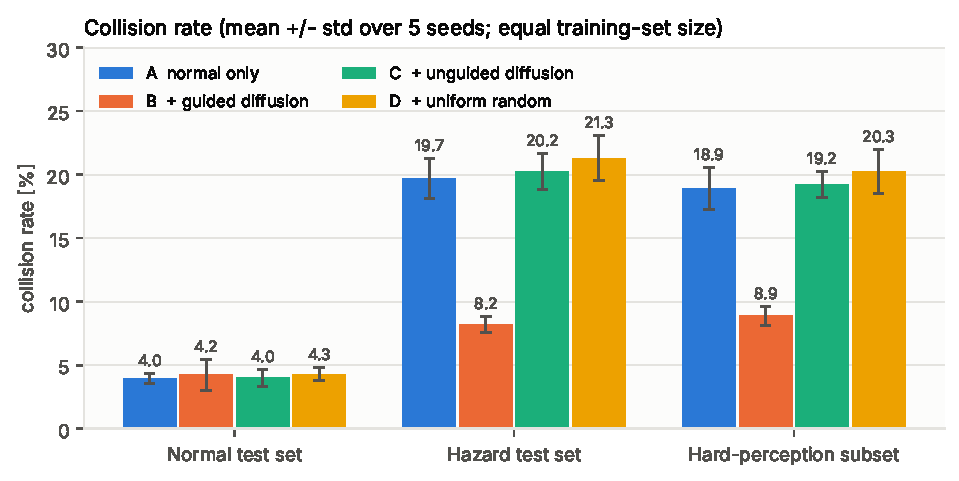
\includegraphics[width=0.88\linewidth]{exp_collision_rates}\\[2pt]
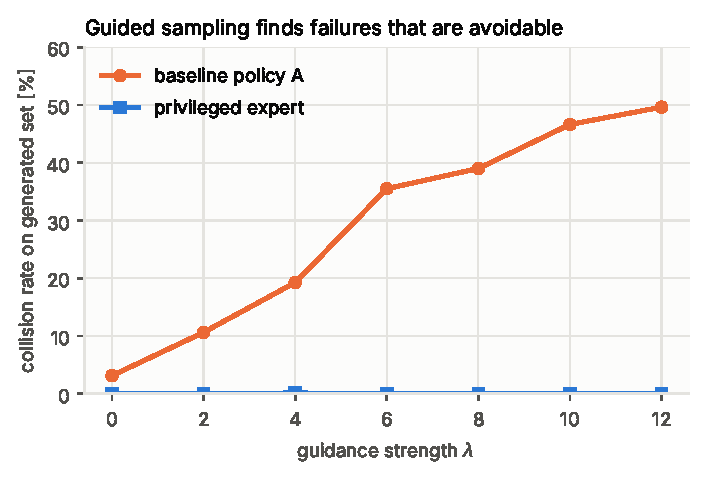
\includegraphics[width=0.48\linewidth]{exp_guidance_sweep}\hfill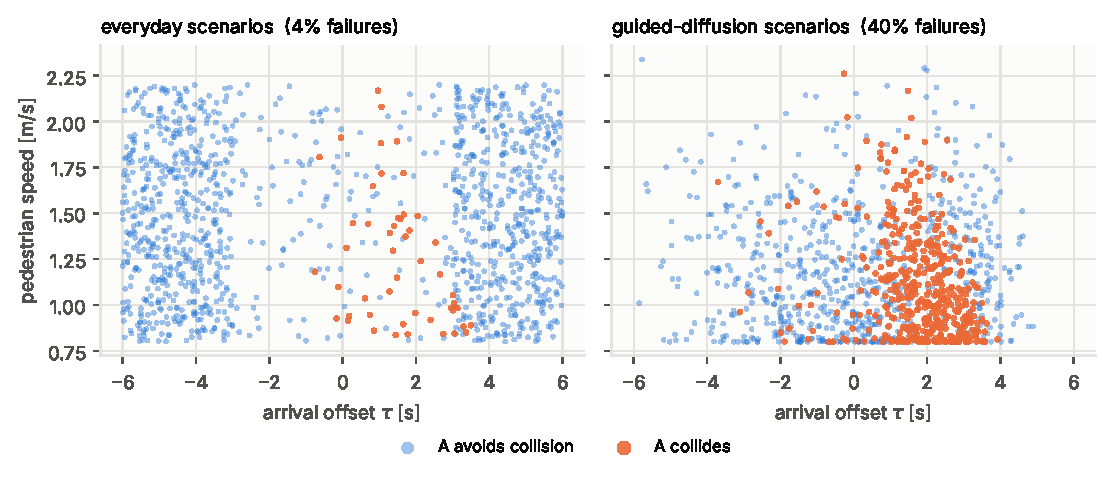
\includegraphics[width=0.5\linewidth]{exp_scatter}
\caption{Top: collision rates. Bottom left: guidance strength $\lambda$ versus failures of policy A on generated sets. Bottom right: where A fails (seed 0).}
\end{figure}
\textbf{Observations.} Only guided data helps ($\collAhazard\to\collBhazard\%$ on hazards); unguided or uniform data of the same size does not (C, D within seed noise of A). Guided scenarios are hard for A (\diagguidedAcoll\% collide) but avoidable (expert \diagguidedExcoll\%). Everyday performance and completion are unchanged. Remaining failures are perception-limited.

\subsection{E2: NeRF-style digital twin}\label{sec:e2}
\textbf{Setup.} 10 expert drives logged (\nerfRays\ rays), field trained \nerfIters\ iterations (\nerfFit\,s); evaluation on 2 unseen drives and on a closed-loop what-if grid (13 pedestrian shifts $\times$ 4 ego speeds) run both in the twin and in the real simulator.
\begin{table}[H]\centering\small
\begin{tabular}{lr}\toprule
Metric & Value\\\midrule
Mean abs.\ range error, held-out views, all rays [m] & $\nvMAE$ (static-only field: $\nvMAEstatic$)\\
Rays within 0.5\,m & $\nvWithin\%$\\
Pedestrian-hit rays ($\nvPedRays$ of $\nvAllRays$): error [m] & $\nvMAEped$ (static-only: $\nvMAEstaticped$)\\
What-if collision outcome agreement ($\wiNcfg$ cases) & $\wiAgree\%$\\
Collision rate real / twin & $\wiCollReal\%$ / $\wiCollTwin\%$\\
Min-gap correlation real vs.\ twin; mean abs.\ difference [m] & $\wiGapCorr$; $\wiGapMAE$\\
Twin without dynamic field: collision rate & $\wiCollNoPed\%$\\\bottomrule
\end{tabular}
\caption{Twin fidelity.}
\end{table}
\begin{figure}[H]\centering
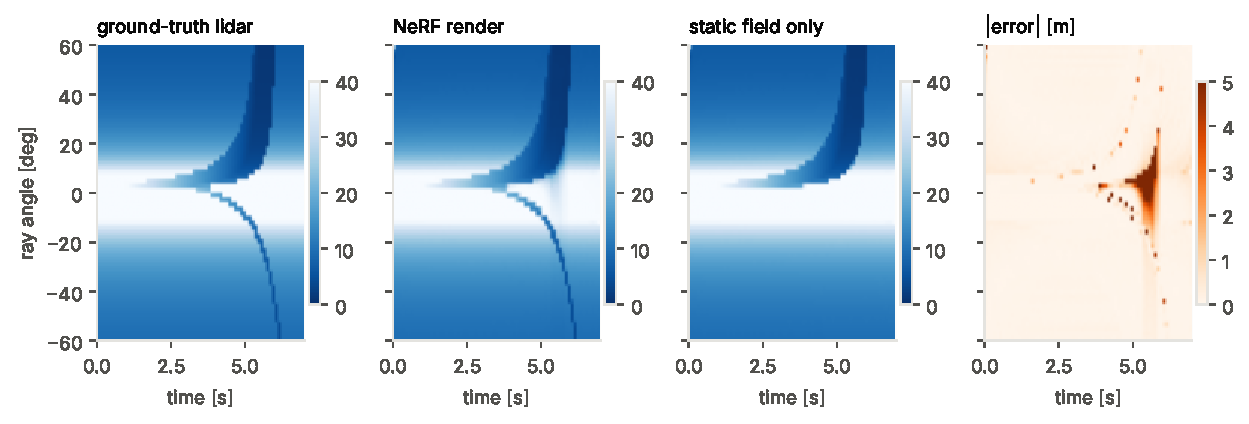
\includegraphics[width=\linewidth]{twin_range_images}\\[2pt]
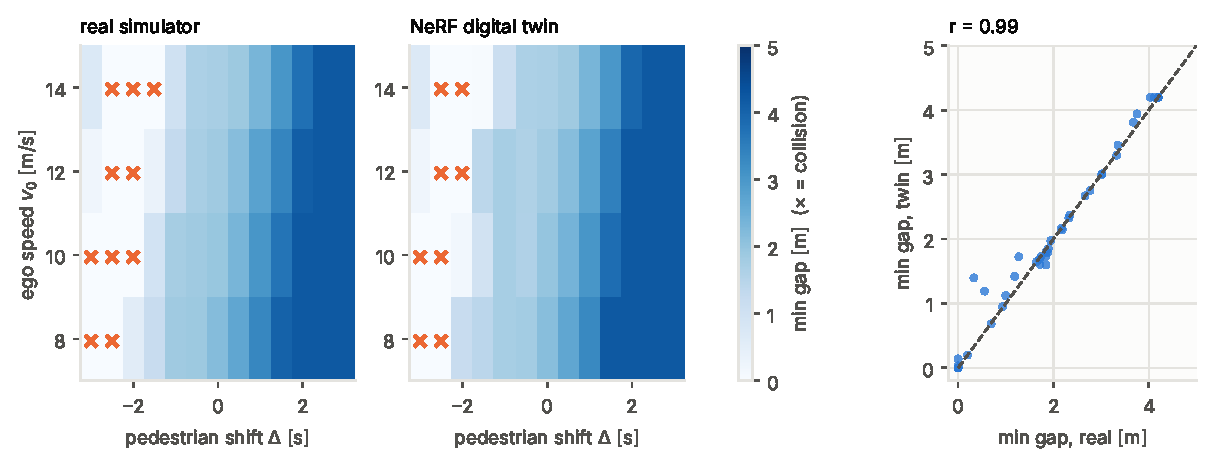
\includegraphics[width=\linewidth]{twin_whatif}
\caption{Top: held-out range images (ground truth, render, static-only, error). Bottom: what-if grid, real simulator versus twin ($\times$ = collision).}
\end{figure}
\textbf{Observations.} The dynamic component is essential: without it the pedestrian is invisible and the policy collides $\wiCollNoPed\%$ of the time. The twin misses fine detail on pedestrian rays (the error panel shows the largest errors late in the drive, when the pedestrian is close to the ego) and reproduces only the logged pedestrian trajectory, shifted in time.

\subsection{E3: Behaviour-tree verification}\label{sec:e3}
\begin{table}[H]\centering\small
\begin{tabular}{ll}\toprule
Property (checked in every abstract state) & Result\\\midrule
P1 action defined and within actuator limits & all hold\\
P2 emergency $\Rightarrow$ full braking $-a_b$ & all hold\\
P3 must-brake $\Rightarrow$ $a\in[-a_b,-0.3]$ & all hold\\
P4 conflict $\Rightarrow$ never accelerate & all hold\\
P5 no conflict $\Rightarrow$ $a\in[-3,2.5]$ & all hold\\
P6 acceleration non-increasing in hazard level & all hold\\\bottomrule
\end{tabular}
\caption{Exhaustive check over $\treeStates$ abstract states (counts per property in \texttt{results/stack.json}).}\label{tab:tree}
\end{table}
\begin{table}[H]\centering\small
\begin{tabular}{llr}\toprule
Tree version & Change & Violations in $\bmcN$\\\midrule
v1 & initial (margins 0/0.5\,s, curb pedestrian assumed safe) & 78 (\texttt{logs/design\_iteration\_1.log})\\
v2 & timing margins only (0.5/1.0\,s) & 276$^\dagger$\\
v3 & + ``yield'' level (never accelerate in conflict) & 78$^\dagger$\\
v4 & + curb pedestrian may start at 3.5\,m/s & 1$^\dagger$\\
v5 (final) & + margins 0.3/0.8\,s & $\bmcViol$ (\texttt{results/stack.json})\\\bottomrule
\end{tabular}
\caption{Bounded model check with true pedestrian state. $^\dagger$Interactive intermediate runs, not archived as files. Of the 78 counterexamples of v1, 75 had a 3.5\,m/s pedestrian: the tree accelerated towards a pedestrian waiting at the curb and could not stop when it started running.}
\end{table}
\textbf{Observation.} Model checking found a real design flaw that unit tests on everyday data had not. Adding margins alone made it worse, which shows the check is not trivially satisfied. The result covers a finite grid with ideal perception only.

\subsection{E4: Planner, optimisation and tracking}\label{sec:e4}
\textbf{Setup.} First 100 hazard scenarios, same lidar perception for BT and planner.
\begin{table}[H]\centering\small
\begin{tabular}{lccc}\toprule
Controller & Collision [\%] & Completed [\%] & Mean min.\ gap [m]\\\midrule
Learned policy A (seed 0) & $\stackAColl$ & $\stackAPass$ & ---\\
Behaviour tree, lidar perception & $\stackBTColl$ & $\stackBTPass$ & $\stackBTGap$\\
Behaviour tree, true pedestrian state & $\stackBToColl$ & $\stackBToPass$ & $\stackBToGap$\\
Lattice + optimiser + PD & $\stackPlColl$ & $\stackPlPass$ & $\stackPlGap$\\
Lattice + optimiser + PD + BT supervisor & $\stackPsColl$ & $\stackPsPass$ & $\stackPsGap$\\\bottomrule
\end{tabular}
\caption{Closed-loop comparison. On all 800 hazard / 800 everyday scenarios the BT with lidar collides in $\btFullHz\%$ / $\btFullNorm\%$.}
\end{table}
\begin{table}[H]\centering\small
\begin{tabular}{lcccc}\toprule
60 hazard scenarios, planner only & RMS tracking error [m] & Collision [\%] & 95th pct.\ jerk [m/s$^3$]\\\midrule
Feed-forward only, nominal brakes & $\trFFRms$ & $\trFFColl$ & $\trFFJerk$\\
PD + feed-forward, nominal brakes & $\trPDRms$ & $\trPDColl$ & $\trPDJerk$\\
Feed-forward only, brake gain 0.8 & $\trFFmRms$ & $\trFFmColl$ & $\trFFmJerk$\\
PD + feed-forward, brake gain 0.8 & $\trPDmRms$ & $\trPDmColl$ & $\trPDmJerk$\\
PD + feed-forward, no optimisation & --- & $\nsColl$ & $\nsJerk$\\\bottomrule
\end{tabular}
\caption{Tracking and optimisation ablations.}
\end{table}
\begin{figure}[H]\centering
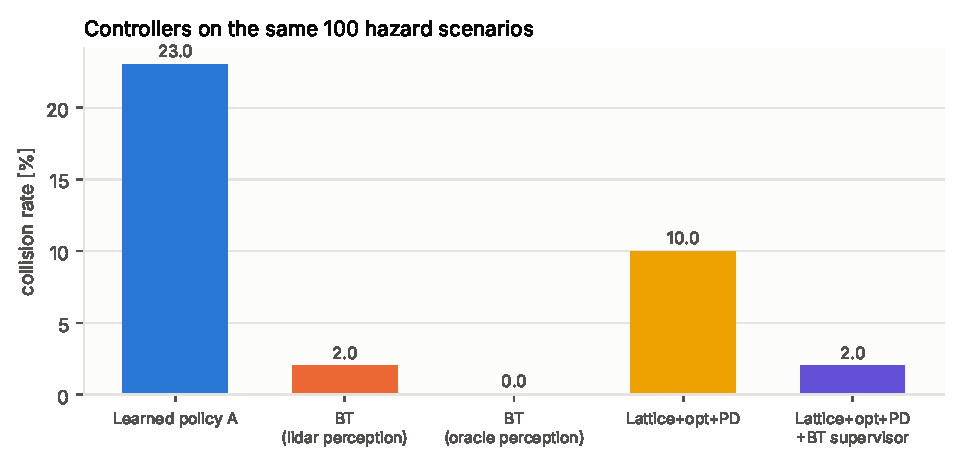
\includegraphics[width=0.62\linewidth]{stack_compare}\\[2pt]
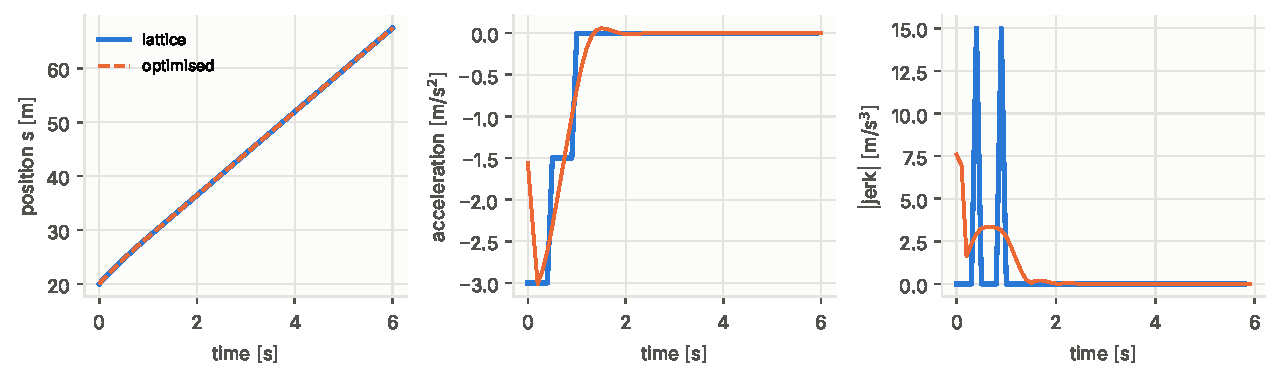
\includegraphics[width=\linewidth]{stack_trajectory}
\caption{Top: controllers on the same scenarios. Bottom: one lattice path versus its optimised refinement (position, acceleration, jerk).}
\end{figure}
\textbf{Observations.} (i) The lattice planner alone collides more than the BT because its pedestrian estimate lags a sudden start; the BT supervisor removes most of this at similar completion. (ii) Optimisation reduces the mean per-plan peak jerk from $\pljerklat$ to $\pljerksm$\,m/s$^3$, but the executed 95th-percentile jerk is essentially unchanged ($\trPDJerk$ with versus $\nsJerk$ without optimisation): replanning every 0.5\,s restarts the profile and the PD term adds step changes, so the smoothing benefit does not reach the vehicle in this configuration. (iii) PD feedback gave no measurable benefit over feed-forward: replanning at 2\,Hz re-anchors the reference to the measured state, so tracking error stays near 6--7\,cm either way; the collision differences in the table are within noise for 60 scenarios. (iv) The learned policy is worst, as in E1.

\subsection{E5: Fault injection}\label{sec:e5}
\begin{table}[H]\centering\small
\begin{tabular}{lcc}\toprule
Fault (400 hazard scenarios) & BT collisions [\%] & BT + monitor [\%]\\\midrule
None (nominal) & $\fNoneplain$ & $\fNonemonitor$\\
Lidar dropout (2\,s) & $\fdropoutplain$ & $\fdropoutmonitor$\\
Frozen frame (2\,s) & $\fstuckplain$ & $\fstuckmonitor$\\
Range bias $\times1.25$ & $\fbiasplain$ & $\fbiasmonitor$\\
Latency 0.3\,s & $\flatencyplain$ & $\flatencymonitor$\\
Brake fade to $-4$\,m/s$^2$ & $\fbrakeplain$ & $\fbrakemonitor$\\\bottomrule
\end{tabular}
\caption{Single-fault injection, lidar perception.}
\end{table}
\begin{figure}[H]\centering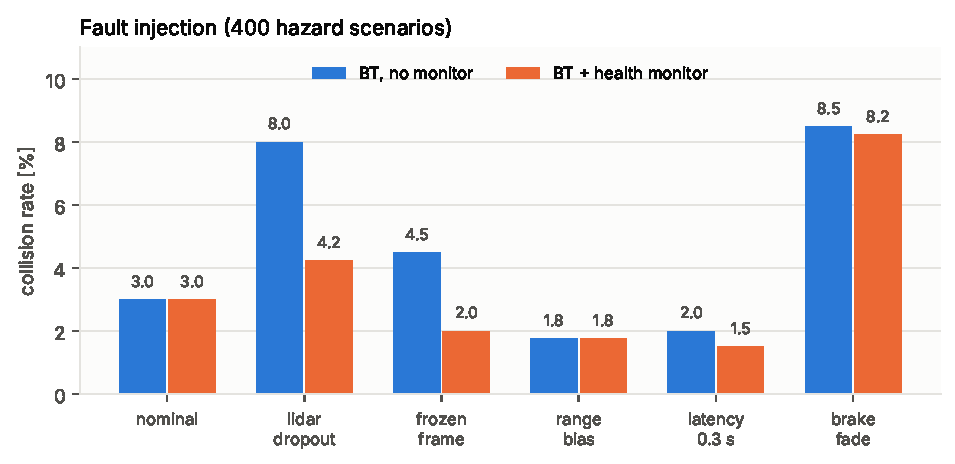
\includegraphics[width=0.82\linewidth]{stack_faults}\caption{Fault injection results.}\end{figure}
\textbf{Observations.} With 400 scenarios the standard error at a 3\% rate is about 0.9 percentage points, so differences below roughly 2 points are not significant. The monitor clearly helps for lidar dropout and frozen frames (about halving collisions). Range bias and latency of this size showed no harmful effect. Brake fade is the one fault that raises collisions markedly, and the monitor does not help: it detects fade only after the first hard braking, which is too late. This is recorded as a residual hazard.

\subsection{E6: Embedded deployment (host CPU)}\label{sec:e6}
\begin{table}[H]\centering\small
\begin{tabular}{lcc}\toprule
Policy ($\embParams$ parameters, $\embMacs$ MACs) & float32 & int8 weights\\\midrule
Latency per inference, gcc -O2, host CPU [\textmu s] & $\embFlns$ & $\embIqns$\\
Code + weights, gcc -Os [KiB] & $\embFlflash$ & $\embIqflash$\\
Max.\ abs.\ difference to NumPy output [m/s$^2$] & \embFlerr{} & \embIqerr{}\\
Collision rate, everyday / hazard set [\%] & $\embFln$ / $\embFlh$ & $\embIqn$ / $\embIqh$\\\bottomrule
\end{tabular}
\caption{C export. Host timings are not microcontroller timings.}
\end{table}
\textbf{Observations.} The generated C reproduces the NumPy policy to float rounding. int8 weights cut code+weights size to about a quarter at a small accuracy cost on hazards; latency is not better on the host because the loop converts int8 to float. On-target cycles are not measured (Sec.~\ref{sec:planned}).

\subsection{E7: Dataset adapter (software test only)}\label{sec:e7}
\texttt{datasets.py} turns KITTI tracking labels into scenario vectors (crossing speed, distance, arrival offset $\tau$). It passes a unit test on a synthetic KITTI-format track with known speed (\texttt{tests.py}). It has \emph{not} been run on real KITTI, nuScenes or Waymo data, which are not reachable from the sandbox.

\section{Safety argument}
Scope: the simulated pedestrian-crossing task (operational domain: straight road, one crossing pedestrian, speeds 6--14\,m/s, pedestrian speed up to 3.5\,m/s, lidar as the only sensor). This is a structured argument linking claims to the evidence above; it is \emph{not} a certified safety case, and no ISO~26262, SOTIF or UL~4600 compliance is claimed.
\begin{table}[H]\centering\small
\begin{tabularx}{\linewidth}{lYYY}\toprule
ID & Claim & Evidence & Residual risk\\\midrule
G0 & The ego avoids collision with a crossing pedestrian in the stated domain & G1--G5 & see below\\
G1 & The BT logic is well-defined and monotone in hazard & E3 exhaustive check, all properties hold & abstraction of continuous state\\
G2 & With correct perception the BT is safe & E3: $\bmcViol$/$\bmcN$ violations; $\stackBToColl\%$ on hazards & finite grid only\\
G3 & Lidar perception is adequate & E4: BT $\stackBTColl\%$ (100 scen.), $\btFullHz\%$ (800) vs.\ $0\%$ with true state & missed or late detections remain\\
G4 & Sensor faults are detected and handled & E5: dropout and frozen frame roughly halved & latency, brake fade not mitigated\\
G5 & An unverified planner cannot override the BT & E4: planner alone $\stackPlColl\%$, with supervisor $\stackPsColl\%$ & supervisor shares the perception\\
G6 & The deployed code equals the tested policy & E6: max.\ difference \embFlerr{} (float32) & int8 changes hazard collisions\\\bottomrule
\end{tabularx}
\caption{Claims and evidence.}
\end{table}
\begin{table}[H]\centering\small
\begin{tabularx}{\linewidth}{lYYY}\toprule
ID & Hazard & Mitigation implemented & Status\\\midrule
H1 & Collision with crossing pedestrian & BT priority levels, curb assumption, margins & mitigated, residual $\btFullHz\%$\\
H2 & Pedestrian hidden by parked car & speed cap 8\,m/s near occluder & mitigated, not eliminated\\
H3 & Lidar dropout / frozen output & health monitor, speed cap 4\,m/s & partly mitigated\\
H4 & Reduced braking & detection by achieved deceleration & \textbf{open}\\
H5 & Sensing latency & none & \textbf{open}\\
H6 & Planner or learned-policy error & BT supervisor (min of accelerations) & mitigated for tested cases\\\bottomrule
\end{tabularx}
\caption{Hazard log.}
\end{table}

\section{Real-world applications}
\begin{table}[H]\centering\small
\begin{tabularx}{\linewidth}{lY}\toprule
Technique here & Industrial counterpart\\\midrule
Spacetime field + what-if replay & neural closed-loop sensor simulation of logged drives (e.g.\ UniSim-style) for regression testing of dangerous events\\
Guided diffusion over scenarios & adversarial and long-tail scenario generation for perception/planner training and validation\\
Verified behaviour tree & runtime safety supervisor / fallback layer next to a learned planner (simplex architecture)\\
Fault injection + monitor & evidence for failure-mode analyses (FMEA/FTA) and degradation strategies\\
C export, int8 weights & deployment of small policies on automotive-grade controllers\\\bottomrule
\end{tabularx}
\end{table}

\section{Experiments planned for this week}\label{sec:planned}
None of these has results yet.
\begin{table}[H]\centering\small
\begin{tabularx}{\linewidth}{lYYY}\toprule
ID & Experiment & Measure & Prerequisite\\\midrule
P1 & Run \texttt{carla\_bt.py} (BT driving a CARLA car, pedestrian crossing) & collision, min gap, comfort vs.\ this simulator & CARLA $\ge$0.9.14 server + \texttt{pip install carla} (code written, unexecuted)\\
P2 & Fit scenario parameters from KITTI/nuScenes pedestrian tracks (\texttt{datasets.py}) and replay in the simulator & distribution of $\tau$, speed, distance vs.\ synthetic prior & dataset download\\
P3 & Time the C policy on a Cortex-M class board & cycles, latency, RAM/flash & board + toolchain\\
P4 & Repeat E3--E5 with 5 seeds and confidence intervals & mean $\pm$ CI for all stack tables & none\\
P5 & Brake-fade mitigation: pre-emptive margin or online decel estimate & collisions under fade & implementation\\
P6 & Latency compensation by state prediction & collisions under 0.3\,s latency & implementation\\
P7 & Larger bounded model check (finer grid, perception-error bounds) & violations & none\\\bottomrule
\end{tabularx}
\end{table}

\section{Future experiments, improvements and observations}
\begin{itemize}[leftmargin=*,itemsep=1pt]
\item \textbf{Perception.} The gap between lidar BT ($\btFullHz\%$) and true-state BT ($0\%$ on the 800-scenario set) is the largest remaining risk. Ray spacing (about 0.7\,m at 20\,m) can miss a 0.5\,m pedestrian; try denser rays or tracking with a motion model.
\item \textbf{Twin.} Move to 3-D camera radiance fields or Gaussian splats; add object-centric dynamic fields so that pedestrian speed and path, not only timing, can be edited.
\item \textbf{Generator.} Guide against the BT as well as the learned policy; add an avoidability filter; extend to multi-agent trajectories.
\item \textbf{Planner.} Longer open-loop execution between replans would test whether PD feedback matters; add lateral motion.
\item \textbf{Embedded.} Quantise activations (full int8), measure on target.
\item \textbf{Observations to keep tracking.} Adding timing margins alone worsened model-check results (E3); a pessimistic default velocity for unseen pedestrians costs some completion time; stack results currently use one seed and 100--400 scenarios, so small differences are not significant.
\end{itemize}

\appendix
\section{Extending this report}\label{app:extend}
\begin{enumerate}[leftmargin=*,itemsep=1pt]
\item Write the experiment as \texttt{code/run\_<name>.py}; save a JSON in \texttt{results/} via \texttt{paths.RES}.
\item In \texttt{code/make\_figures\_stack.py} add \texttt{mac("name", value)} lines (letters only in macro names) and any figure.
\item Copy a block in \texttt{sections/04\_experiments.tex} (setup, table, figure, observations), move the row in Table~1 and in Sec.~\ref{sec:planned} from \planned\ to \done.
\end{enumerate}
\paragraph{Reproducibility.} All runs are seeded; \texttt{results/} and \texttt{figures/} shipped with this folder were produced by \texttt{make results figures} in a 2-core sandbox (NumPy, Matplotlib). Latencies in E6 depend on the machine.

\section{Source code}\label{app:code}
\newcommand{\code}[3]{\subsection{\texttt{#2}}\lstinputlisting[style=py]{code/#1}\label{#3}}
\code{paths.py}{paths.py}{c:paths}
\code{nn.py}{nn.py}{c:nn}
\code{sim.py}{sim.py}{c:sim}
\code{driving.py}{driving.py}{c:driving}
\code{scenario_gen.py}{scenario\_gen.py}{c:gen}
\code{nerf2d.py}{nerf2d.py}{c:nerf}
\code{stack.py}{stack.py}{c:stack}
\code{datasets.py}{datasets.py}{c:data}
\code{carla_bt.py}{carla\_bt.py}{c:carla}
\code{embedded.py}{embedded.py}{c:emb}
\code{run_experiments.py}{run\_experiments.py}{c:rune}
\code{run_twin.py}{run\_twin.py}{c:runt}
\code{run_stack.py}{run\_stack.py}{c:runs}
\code{make_figures.py}{make\_figures.py}{c:mf}
\code{make_figures_stack.py}{make\_figures\_stack.py}{c:mfs}
\code{tests.py}{tests.py}{c:tests}
\subsection{\texttt{Makefile}}\lstinputlisting[style=plain]{Makefile}

\end{document}
